\chapter[SCP-149 血蝇]{
    SCP-149 The Blood Flies\\
    SCP-149 血蝇
}

\label{chap:SCP-149}

\begin{figure}[H]
    \centering
    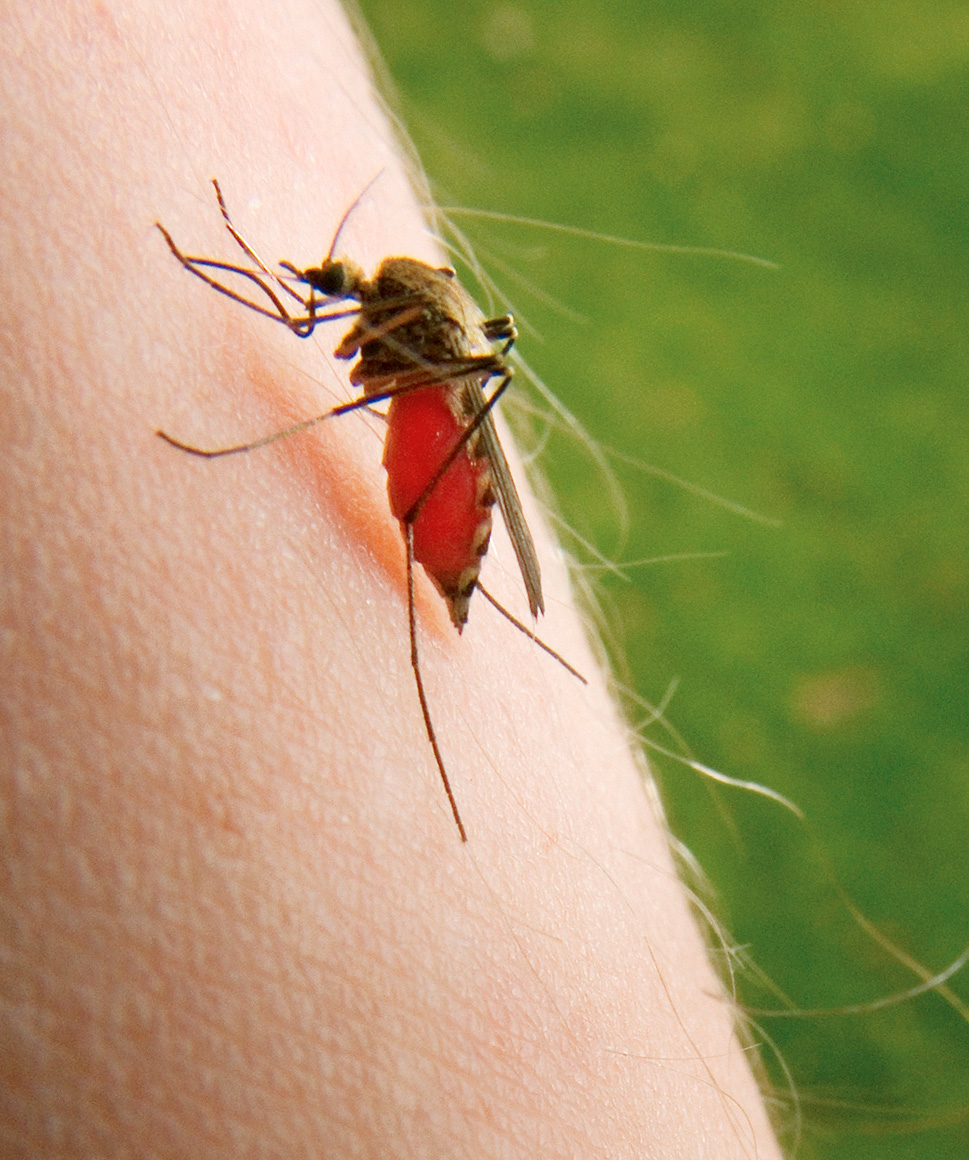
\includegraphics[width=0.5\linewidth]{images/SCP.149.jpg}
    \caption*{SCP-149 正感染一名 D 级测试对象。}
\end{figure}

\bb{项目编号:}SCP-149

\bb{项目等级:}Keter

\bb{特殊收容措施:}任何SCP-149样本需要放置在密封树脂玻璃盒中观察。每隔两小时需要向隔离室中输送氧气和雾化营养液。149-1号事故后,O5-12规定若有SCP-149样本从隔离室逃离,任何受感染的人员需要依照42-查理协议进行处理。

\bb{描述:}SCP-149这种蚊子携带一种逆转录酶病毒(称为SCP-149-A),它能使人类细胞变异为蚊子的受精卵。SCP-149在叮咬时会将SCP-149-A直接注入血液,后者会迅速作用细胞核,使DNA扭转变型。首批依照错误的遗传指令繁殖的细胞酷似囊肿,并在食道和鼻窦内膜中聚集。解剖结果显示,这些“囊肿”充满了SCP-149的幼虫,而“囊肿”本身则是一个抵御外力的保护层。SCP-149度过成熟期只须数小时;当受试者感到不适,第一代SCP-149已经在受试者体内发育成熟。SCP-149主要从寄主的口腔和鼻孔离开,偶尔也取道蝶窦从眼眶离开。被SCP-149感染足以致命,估计一次叮咬的感染机率为50\%。

\bb{附录:}

149-1号事故:SCP-149意外出逃并感染了多名D级人员,他们大多数并未报告与SCP-149有过接触。不到5小时,SCP-149已发育成熟并从寄主体内喷出,感染了███名员工。幸好██████医生反应迅速,及时封锁了地下12层至15层,现场才没有遭到彻底的污染。据这次事件,O5提出了42-C协议,用于SCP-149逃脱管制的情况。
